\section{Développement du logiciel}
\subsection{Développement avec boost}
\subsubsection{Des difficultés de prise en main}
La prise en main de \textit{Boost} a été la principale difficulté du projet. En effet, la documentation fournie avec la librairie, disponible sur le site officiel, ne ressemble en rien aux documentations de la stl ou de java... C'est d'autant plus difficile que la philosophie de développement de \boost est assez éloignée de ce que nous connaissions juqu'alors et finalement assez éloignée de la programmation objet (pour la partie graph) : la plupart des méthodes que nous utilisons sont en fait des fonctions.

Pour trouver les fonctions relatives aux objets, ou comment les utiliser, il faut parcourir une dizaine de pages web de documentation par fonction expliquant comment les appeler i.e. : comment créer les structures adéquates, quels arguments et structures passés en paramètres et comment les créer... Cette documentation n'est pour autant pas exhaustive et manque cruellement d'exemples, elle est clairement destinée à un public d'experts.

\subsubsection {Compilateur spécifique}
Les erreurs retournées par gcc à la compilation de la librairie sont incompréhensibles, c'est pourquoi il faut utiliser un compilateur particulier. \verb|gfilt| est compilateur utilisant perl pour analyser les erreurs de compilation et afficher des erreurs intelligibles. 

Malheureusement, il n'est pas possible de compiler Qt avec ce compilateur. Nous avons donc créé un dossier de développement spécifique à \textit{Boost} que nous mergions avec la partie Qt quand nous étions satisfaits du résultat. La solution la plus efficace aurait été de créer une branche sous git, mais nous n'avions pas encore décidé d'utiliser git lorsque nous avons rencontré ce problème.

\subsubsection{Bilan}

Tout au long du projet, la méthode la plus efficace pour avancer lorsque nous bloquions sur \boost a été de demander l'éclairage de notre tuteur de projet. 

\textit{Boost} est une librairie véritablement complexe dans sa construction, son code, sa compilation et son fonctionnement. L'utilisation massive des génériques et de la méta-programmation peut rendre la compilation relativement longue mais améliore grandement les performances.
~\\
Un exemple d'utilisation  concrète de \textit{Boost}, des difficultés dûes au côté ``non objet'' de la partie graphe et de ses apports en terme de performance est le traitement du fichier contenant la ``table de routage d'internet''.

\subsection{Décodeurs d'entrée}
Le fichier contenant les liens entre les AS est une succession de lignes ``\verb|AS1 AS2 TYPE|'' représentant le lien entre l'AS1 et l'AS2 et son type. Or nous nous ne souhaitons conserver que le numéro de l'AS. C'est à dire une ligne de type ``\verb|1 2 TYPE|''. C'est pourquoi, la première étape lorsque nous récupérons un fichier de données est d'effectuer un traitement à l'aide de sed (figure \ref{sed}) afin de retirer les ``\verb|AS|'' et d'accélérer les traitements lors de la lecture du fichier. 
\begin{figure}[H]
   \begin{center}
      \begin{tabular}{l}
         \hline
         \verb|sed -i -e "s/AS//g" nom_du_fichier|\\
         \hline
      \end{tabular}
   \end{center}
\caption{\label{sed} Ligne de commande du traitement de sed}
\end{figure}

L'étape de lecture à proprement parler peut commencer une fois ce pré-traitement effectué par l'utilisateur. 

\subsubsection{Méthode C++}

Au début du projet, nous avons utilisé une méthode ``C++'' classique pour lire et parser le fichier. 
Représenté en figure \ref{parse_cpp}, le parsing dit classique est beaucoup moins performant que le parsing de boost, en outre il augmente considérablement le nombre de \verb|if| imbriqués ce qui rend le code plus difficile à lire, il faut ajouter autant de \verb|else| pour la gestion des erreurs qui a été retirée du présent rapport. L'avantage de cette méthode est que nous récupérons directement \verb|asn1| et \verb|asn2| les numéros des AS correspondant à la ligne du fichier en cours de lecture en tant qu'entier.

\begin{figure}[H]
   \begin{center}
      \begin{tabular}{l}
        \hline 
        \verb|std::ifstream file(filename.c_str());|\\
	\verb|if( file.is_open() )|\\
	\verb|{|\\
   	\verb|    while(std::getline(file, line)) {|\\
      	\verb|    std::istringstream lineStream(line);|\\
      	\verb|    if(lineStream >> tempString) {|\\
        \verb|        std::istringstream in1(tempString);|\\
        \verb|        if(lineStream >> tempString) {|\\
        \verb|            std::istringstream in2(tempString);|\\
        \verb|            //Si tout rentre dans chacun des conteneurs...|\\
        \verb|            if(lineStream >> linkType && in1 >> asn1 && in2 >> asn2) {|\\
        \verb|                //TRAITEMENT|\\
        \verb|           }|\\
        \verb|        }|\\
        \verb|    }|\\
        \verb|}|\\
        \hline
      \end{tabular}
   \end{center}
\caption{\label{parse_cpp} Exemple de parsing de fichier en C++ classique}
\end{figure}




\subsubsection{Méthode Boost}
Le parsing avec boost utilise un \verb|tokenizer| et un \verb|char_separator| qui permet de décrire à boost comment parser la chaine qu'il reçoit en entrée. Représentée en figure \ref{parse_boost}, Cette méthode de découper les fichiers est beaucoup plus performantes que celle du C++ classique. Si la ligne n'est pas conformé à nos critères la taille du vector de string est différente de 3 et nous retournons une erreur (ici non représentée). 

Contrairement à la version C++, si la ligne est découpée correctment, nous ne récupérons pas directement des entiers. Heureusement boost dispose d'outils de ``cast'' très performant, qui permettent notamment de ``caster'' un \verb|string| en \verb|int| (figure \ref{cast_boost}) sans pertes de performances visibles. A titre d'exemple, la méthode C++ classique prenait environ 8 secondes à s'exécuter, tandis que celle de boost ne prend plus que 4 secondes, les deux mesures contiennent les traitements et ont été exécuter sur un fichier d'environ 150000 lignes...

Au final, le traitement d'une ligne se déroule comme présenté figure \ref{file_parser}. Nous nous servons d'une map de traduction qui permet de trouver quel AS est déjà présent dans le graph et de récupérer son \verb|vertex_descriptor|. En effet, chaque \verb|vertex_descriptor| est un entier mais il ne correspond pas au numéro de l'AS en question. Utiliser le numéro de l'AS comme \verb|vertex_descriptor| reviendrait à créer des AS fantômes, le graphe serait donc trop gros et surtout la représentation graphique et les données correspondants aux AS seraient éronnées.

Les fonctions utilisées pour ajouter des sommets et des arêtes (\verb|add_vertex| et \verb|add_edge|) au graphe montrent, encore une fois, que la partie graphe de boost est assez éloignée de l'objet.

\begin{figure}[H]
   \begin{center}
      \begin{tabular}{l}
        \hline 
 	\verb|typedef boost::tokenizer< boost::char_separator<char> > tokenizer;|\\
 	\verb|boost::char_separator<char> sep("\t");|\\
	\verb||\\
	\verb|std::ifstream file(filename.c_str());|\\
	\verb|if( file.is_open() )|\\
	\verb|{|\\
	\verb|    while(std::getline(file, line)) {|\\
	\verb|        tokenizer tokens(line, sep);|\\
	\verb|        std::vector<std::string> parts(tokens.begin(), tokens.end());|\\
	\verb|        if( parts.size() == 3)|\\
	\verb|        {|\\
	\verb|            //TRAITEMENT|\\
	\verb|        }|\\
	\verb|    }|\\
	\verb|}|\\
        \hline
      \end{tabular}
   \end{center}
\caption{\label{parse_boost} Exemple de parsing de fichier en C++ avec boost}
\end{figure}
 

\begin{figure}[H]
   \begin{center}
      \begin{tabular}{l}
        \hline 
 	\verb|asn1 = boost::lexical_cast<int>(parts.at(0));|\\
        \hline
      \end{tabular}
   \end{center}
\caption{\label{cast_boost} Exemple de ``cast'' avec les outils de boost}
\end{figure}

\begin{figure}[H]
\begin{center}
        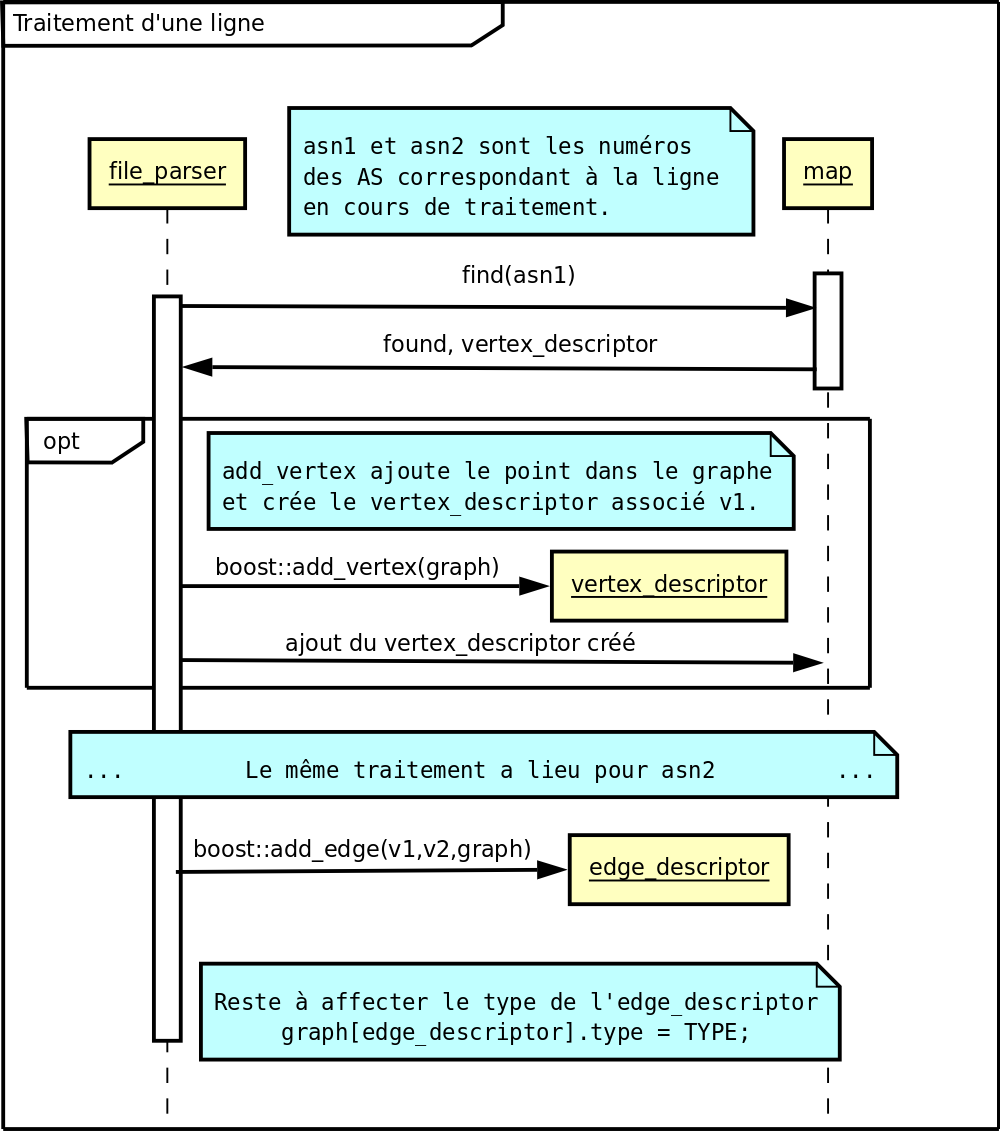
\includegraphics[width=0.7\textwidth]{./schema/file_parser2.png}
\caption{``Diagramme de séquence'' du parsing d'une ligne }
\label{file_parser}
\end{center}
\end{figure}

\subsubsection{Gestion des erreurs}

La gestion des erreurs lors du parsing du fichier se fait de manière un peu particulière. Afin de rendre le bloc parsing de fichier totalement indépendant du reste, nous avons choisi d'utiliser un simple booléen qui indique si une erreur s'est produite à cause de la lecture d'une ligne, dans le cas où l'erreur est critique (fichier inexistant, illisible ou toutes autres raisons de ce type), un autre type d'erreur est détectée. 

Pour signaler, l'erreur à la couche supérieure (le controlleur), nous remontons une exception \verb|ReaderException| de nature \verb|CRITICAL| n'importe quand ou \verb|NON_BLOCKING| une fois le graphe rempli de maniètre à empêcher ou non l'exécution de la suite du code.


\subsection{D\'eveloppement avec Qt}

\par
Le developpement avec Qt s'est fait \`a l'aide de la documentation tr\`es fournie du site de \textit{TrollTeech}. Celui propose un aper\c cu des diff\'erentes classes, ainsi qu'un certain nombre d'exemples pour aider les d\'eveloppeur.
\par
La principale difficult\'e de d\'evelopper avec Qt r\'eside dans la compr\'ehension des slots et signaux. Ce sont eux qui font toute l'interactivit\'e d'une interface graphique. Pour rendre op\'erationnelle une entr\'ee dans un menu, il faut connecter l'action qu'elle repr\'esente au slot correspondant dans son objet parent.
\par
Notre fen\^etre principale contient donc les d\'eclarations des actions correspondant aux diff\'erentes entr\'es des menus, par exemple sur la figure \ref{exemple_action_qt}, on voit la d\'eclaration de l'action permettant de quitter le programme en fermant toutes les fen\^etres.
\begin{figure}[H]
   \begin{center}
      \begin{tabular}{l}
         \hline
         \verb|QAction * _quitAct;|\\
         \hline
      \end{tabular}
   \end{center}
\caption{\label{exemple_action_qt} Exemple de d\'eclaration d'action Qt}
\end{figure}
Ensuite, lors de l'initialiation de la fen\^etre, il faut associer les 
entr\'ees du menu \`a une action, ce qui est pr\'esent\'e figure \ref{exemple_menu_qt}.

\begin{figure}[H]
   \begin{center}
      \begin{tabular}{l}
         \hline
         \verb|_fileMenu.addAction(_quitAct);|\\
         \hline
      \end{tabular}
   \end{center}
\caption{\label{exemple_menu_qt} Exemple de d'association d'action Qt \`a une entr\'e d'un menu}
\end{figure}

Enfin, il faut associer l'action \`a un slot d'un des \'el\'ement du programme si on veut que cela fasse quelque chose lorsque l'on clique sur l'entr\'e du menu. Figure \ref{exemple_initAction_qt}, on peut voir que l'action est d'abord cr\'e\'ee avec un nom, et attach\'ee \`a un objet, ici \textit{this} fait r\'ef\'erence \`a la fen\^etre principale. On assigne ensuite un raccourcis et une description \`a l'action. Finalement, l'\'etape la plus importante, on connecte l'action au slot de fermeture de la fen\^etre principale.

\begin{figure}[H]
   \begin{center}
      \begin{tabular}{l}
         \hline
         \verb|_quitAct = new QAction("Quit", this);|\\
         \verb|_quitAct->setShortcut(tr("Ctrl+Q"));|\\
         \verb|_quitAct->setStatusTip("Quit the program");|\\
         \verb|QObject::connect(_quitAct, SIGNAL(triggered()), this, SLOT(close()));|\\
         \hline
      \end{tabular}
   \end{center}
\caption{\label{exemple_initAction_qt} Exemple d'initialisation d'un action Qt}
\end{figure}

Ces \'etapes doivent \^etre r\'ealis\'ees pour toutes les actions. Il est \`a noter que l'on peut d\'eclarer \`a volont\'e des slots dans un objet. Ces slots sont en r\'ealit\'es des fonctions qui ne sont d\'eclar\'ee ni en \textit{public}, \textit{private} ou \textit{protected} mais en tant que \textit{slots} (qui peuvent \^etre publics ou priv\'es). On peut ainsi cr\'eer des fonctionalit\'es comme bon nous semble pour le programme.

\par
Lors de la cr\'eation d'un objet Qt, on utilise un macro : \verb|Q_OBJECT| qui permet la gestion des slots et signaux au moment des diff\'erentes \'etapes de la compilation.

\par
Voici l'exemple de la classe \verb|mainWindow| de notre programme qui est la fen\^etre  principale de l'interface graphique :

\begin{figure}[H]
   \begin{center}
      \begin{tabular}{l}
         \hline
         \verb|public class mainWindow : public QMainWindow|\\
\verb|{|\\
\verb|    Q_OBJECT|\\
         \verb|    protected :|\\
         \verb|        //...les attributs de la classe...|\\
         \verb|    public :|\\
         \verb|        //...les méthodes publiques de la classe...|\\
         \verb|    public slots :|\\
         \verb|        //...les slots publiques de la classe...|\\
\verb|}|\\
         \hline
      \end{tabular}
   \end{center}
\caption{\label{exemple_mainWindow_qt} Exemple d'un classe Qt}
\end{figure}

La classe mainWindow h\'erite de la classe QMainWindow de Qt qui est la classe pour les fen\^etres principales d'un programme dans laquelle, on ajoute tous les \'el\'ements composant le programme (menu, zone de dessin, barre de statut) sous forme d'attributs de classe.
Un certains nombre de m\'ethodes publiques sont d\'efinies pour int\'eragir avec ces \'el\'ements, par exemple : changer tel ou tel affichage dans la zone de dessin.
Enfin, un certain nombre de slots publiques correspondent aux actions r\'ealisables dans les menus. Ces slots sont des fonctions qui sont appel\'ees en r\'eponse \`a un clique de souris sur un menu ou un bouton.

\subsection{Expérimentation sur le code}
Notre connaissance grandissante des librairies utilisées nous a permis de pratiquer diverses expérimentations sur nos algorithmes, traitements et affichages.
\subsubsection{Expérimentation avec Qt}
\paragraph{}
Au cours de la premi\`ere phase du projet, nous avons un module de lecture sur fichier vraiment lent, aussi, il arrive souvent lors du chargement du fichier que notre fen\^etre principale devienne grise. En effet, l'OS cherche \`a signifier par l\`a que la fen\^etre ne répond plus depuis un moment, ce qui \'est normal vu les traitements que le programme r\'ealise en arri\`ere plan.
Aussi nous d\'ecidons d'afficher une petite fen\^etre annon\c cant que le calcul est en cours. Pour cela, nous effectuons des recherches sur les \textit{QThread}. Ceux-ci doivent permettre \`a notre fen\^etre de chargement de continuer d'\^etre active m\^eme si la fen\^etre principale ne r\'epond plus.
Nos recherche nous apprennent que l'on ne peut g\'erer de l'affichage en dehors du thread principal en Qt. Donc, pour afficher une fen\^etre de chargement, elle doit être g\'er\'ee par le m\^eme thread que la fen\^etre principale. Ce sont les calculs qui doivent \^etre effectu\'es par un autre thread.
Avec l'arriv\'ee du second module de lecture de fichier, le processus est devenu plus rapide et l'utilit\'e de cette fen\^etre pour faire patienter l'utilisateur nous semble moins importante, aussi l'id\'ee est rel\'egu\'ee au second plan, et finalement ne se retrouve pas impl\'ement\'ee dans le programme final.

\subsubsection{Expérimentation avec boost}

\paragraph{Kamada Kawai Layout}
Kamda Kawai Layout est une fonctions de \boost permettant de calculer les coordonn\'ees des points d'un graphe. Contrairement \`a Circle Graph Layout qui les pla\c ce sur un cercle, Kamada kawai les organise selon leur poids.
Kamada Kawai n\'ecessite un graphe connexe, ce qui n'est pas le cas de la topologie IPv6, aussi cette fonction n'est pas impl\'ement\'ee dans la version finale.

\paragraph{Recherche des peers\\}
\par La recherche des peers a été développé en deux étapes. La première étape fut de trouver un moyen de recenser les Peers à partir de fichier de routage uniquement, afin de permettre de trouver les cliques avec un algorithme ``maison''. Cette méthode se basait sur le ciblage des AS qui n'avaient ni client, ni peer : ce sont n\'ecessairement des stubs. A ce moment là, nous stockions plusieurs graphs dans l'objet contrôleur dont le principale et celui sans les stubs.

Cette méthode présupposait que le fichier était ordonné et bien que ce soit le cas avec le fichier qui nous servait de base cela ne le serait pas forcément avec tous les fichiers devant être utilisés. Et ordonner manuellement un fichier de 100000 lignes reléverait d'un exploit digne d'un héros de la mythologie grecque. Ordonner ce fichier avec une fonction dédiée était possible, mais il fallait trouver un moyen plus ``propre'' et performant.

\par Notre tuteur de projet, Monsieur Meulle, nous a fourni un nouveau fichier, avec des relations entre AS sous la forme de triplets, permettant d'identifier tr\`es rapidement les AS feuilles.
Les liens entre AS sont plac\'ees sous la forme : {AS1, AS2, AS3} signifiant que pour joindre l'AS3, l'AS1 a dû passer par l'AS2. Les AS du milieu sont donc forcément des AS de transit, les AS stubs sont alors facilement identifiables comme \'etant tous les autres... 

C'est à ce moment-là que le structure actuelle du programme a été clairement établie, nous ne stockons qu'un seul graphe dans le controlleur et celui-ci réalise un traitement de création d'un graphe spécifique en fonction de ce qui lui ait demandé. Un fonctionnement proche d'une base de données décrit en \ref{mvcText}. 

En outre, l'utilisation du modèle MVC nous a permis de continuer à travailler sur l'ensemble du projet. Pendant que l'un d'entre nous apportait les corrections nécessaires à la partie lecture de fichier, l'autre continuait de développer l'interface graphique. La fusion des deux parties s'est révélée triviale le contrôleur ne perdant pas de fonctionnalités, il ne restait plus qu'à l'adapter et à lui en ajouter de nouvelles.
